There are many types of neural networks and each of them perform differently according to the task. Considering the low vocabulary of our task and the large amount of data, we'll be looking to search for patterns through the identification of templates with neural networks. Therefore, CNN comes immediately to mind. But many works suggests the use of recurrent neural networks. Therefore we'll focus on those two types of networks that seems to be the most promising. Finally, MLPs are usually mentionned but not for their performances, mostly because they are easy to implement and it's always a nice comparison.

\vspace{5mm}

Keyword spotting task are extremely fit to CNNs according to many research \cite{CNN}, \cite{init}. A DNN cannot take advantage of the topology of the signal, however CNNs are extremely good at acoustic modeling which permits to give a good representation of a speech spectrum. The differences of frequencies between each speaker and also the timing differences between each examples are known to be easily handled by CNNs.

\vspace{5mm}

RNNs and especially LSTMs are also fit to this task because of their ability to take into account time sequences through feedback connections. They also benefits from the combination of lstm layers with deep or convolutionnal layers \cite{graves}. But one of the main problem encountered with RNNs, is that they are slow for many reasons (no parrellelization, slow learning, ...). Therefore the trend is to move away from recurrent structures.



\section{MLP}

Neural networks are used to approximate functions which solving a non linear optimization problem that tries to find the minimum "distance" between the approximation and the real function. To do so, training algorithms try to find the set of weights that minimize the "distance" represented by the loss function.

\vspace{5mm}

MLPs are one of the most simple form yet usually reliable of neural networks. They are composed of one input layer, one output layer and at least one hidden layer. They are feed forward that means that the flow of information goes in only one direction : from input layer to output layer.


\section{CNN}
CNNs are an evolution of MLPs. Indeed, usually they have an MLP base that is situated at the end of the network but they also have some convolutions layers. the role of those convolution layers will be to split the input in order to find interesting information in a small subset of it. This will make CNN be able space dependecies in 2-d data. In addition of that, CNNs are usually more effective than MLPs in term of computation. 

\section{LSTM}

LSTM structures (Long short term memory) are a chain like network where you gives the output of a block as an input of the next one. The idea being similar to recurrent neural networks, it's about creating an artificial memory of how inputs evoluate over time. It is extremely interesting for tasks with temporal dependencies such as speech recognition. The improvement over the RNN structures is the forget gate that allows to manipulate weights of recurrents connections in order to face the vanishing gradient problem. Therefore 

\begin{figure}[h!]
    \centering
    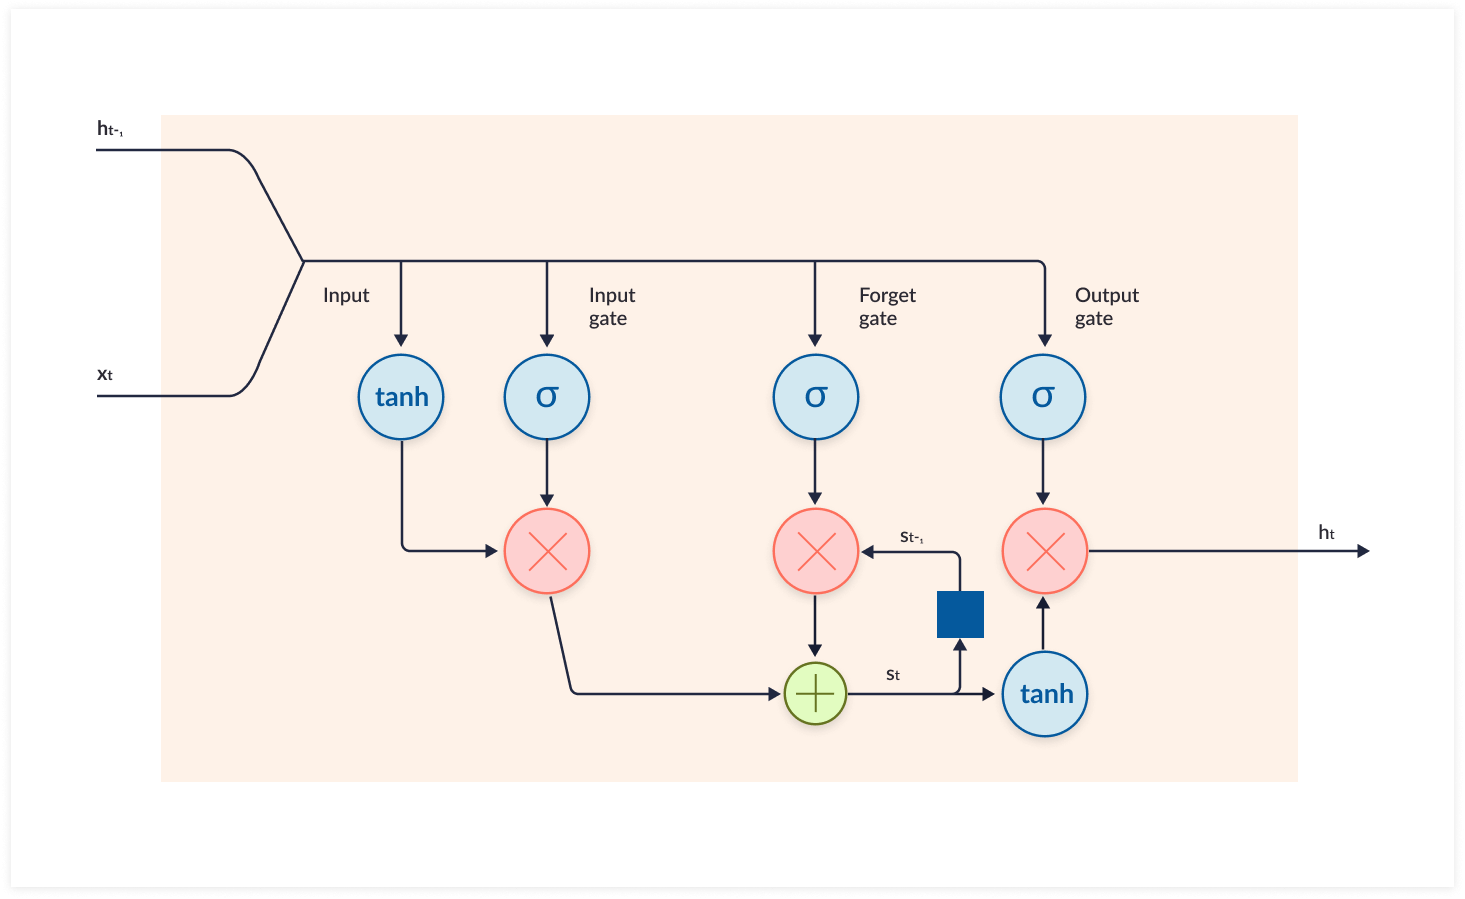
\includegraphics[width=1\textwidth]{chapters/pictures/lstm_unit.png}
    \caption{Inside of a LSTM unit}
    \label{fig:mlp}
\end{figure}
